\chapter{実現} \label{implementation}

\simname は Python を用いて実現されている。入力と表示に Jupyter Notebook~\cite{kluyver_jupyter_nodate} 、グラフの描画に matplotlib~\cite{hunter_matplotlib_2007} 、方程式の処理や数値計算に SymPy~\cite{meurer_sympy_2017} を用いている。

\begin{figure}[htb]
\centering
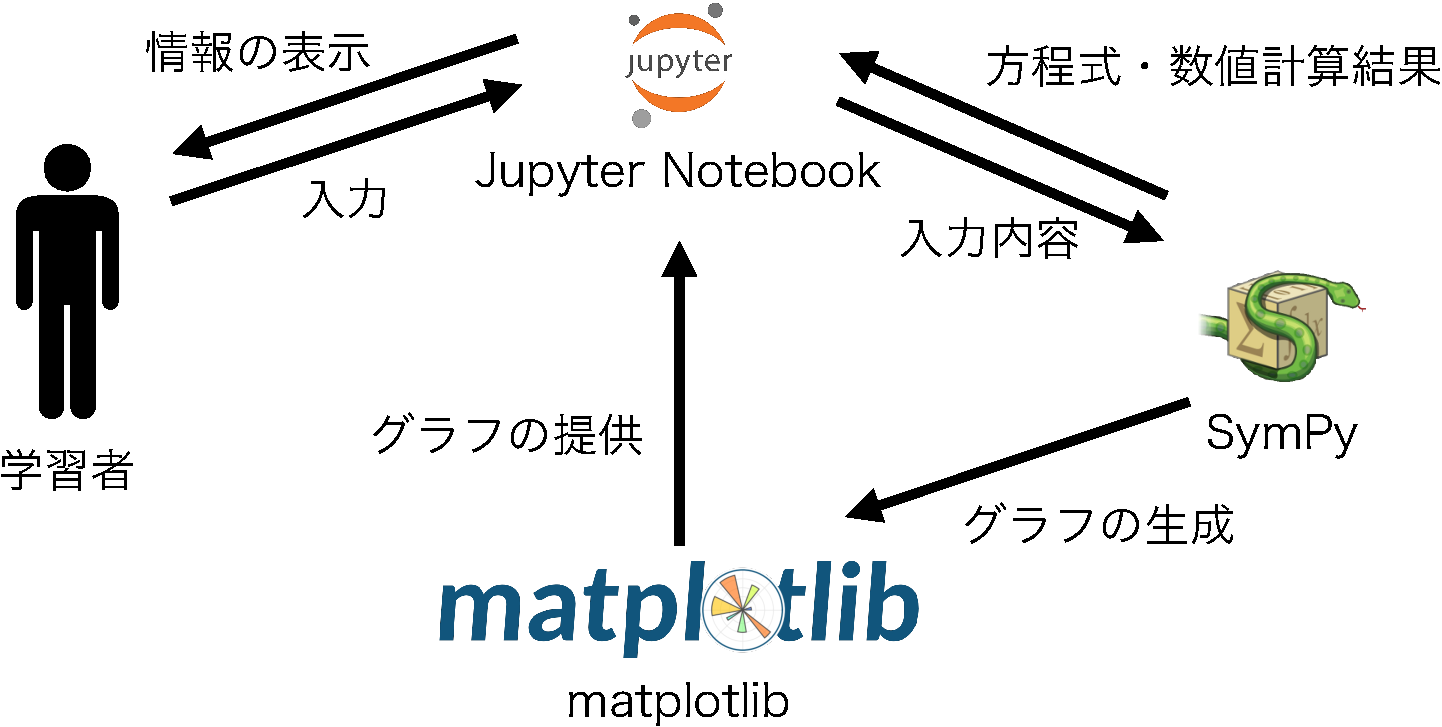
\includegraphics[width=0.8\linewidth]{work/imple_diagram-crop.pdf}
\caption{簡単な全体像}
\end{figure}

\section{使用している道具}

\subsection{Jupyter Notebook}
Jupyter Notebook は IPython~\cite{perez_ipython_2007} から分離したプロジェクトで、Jupyter Notebook から IPython カーネルを呼び出すことで、Python のコードを対話的に実行することができる。また、ipywidgets ライブラリを利用すると、Jupyter Notebook 上に GUI を作成することができる。図~\ref{example_jupyter}は、Jupyter Notebook 上にクリックすることのできる Button と、文字を入力できる Text の Widget を生成する例である。

\begin{figure}[htb]
\centering
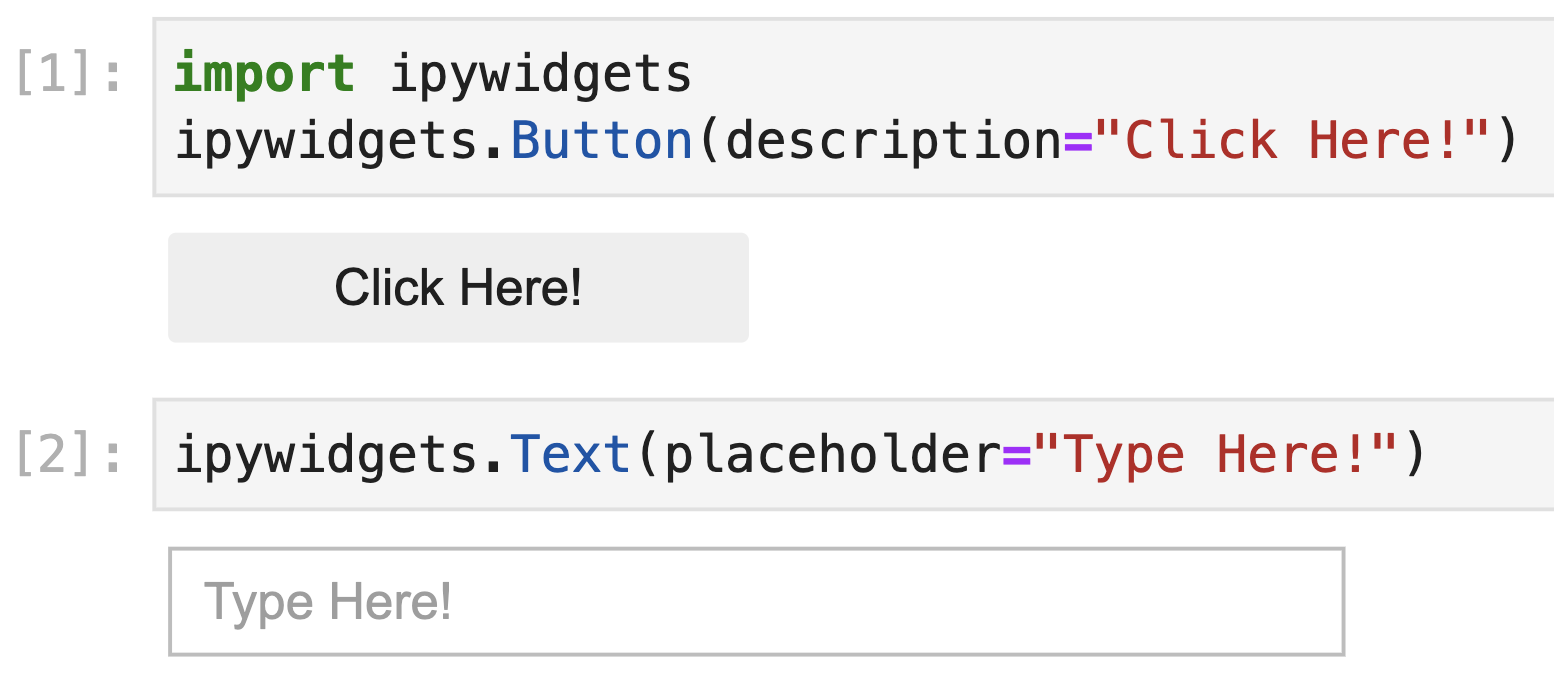
\includegraphics[width=0.9\linewidth]{work/example_jupyter.png}
\caption{Jupyter Notebook 上に Button と Text の
Widget を生成する例} \label{example_jupyter}
\end{figure}

\subsection{matplotlib}
matplotlib は、グラフを描画するためのライブラリである。Jupyter Notebook 上で matplotlib を用いると、グラフを Jupyter Notebook に表示することができる。また、出力先として ipywidgets の Output を用いることで、ipywidgets で作成した GUI にグラフを組み込むことができる。図~\ref{example_matplotlib} は matplotlib を用いて簡単なグラフを描画する例である。

\begin{figure}[htb]
\centering
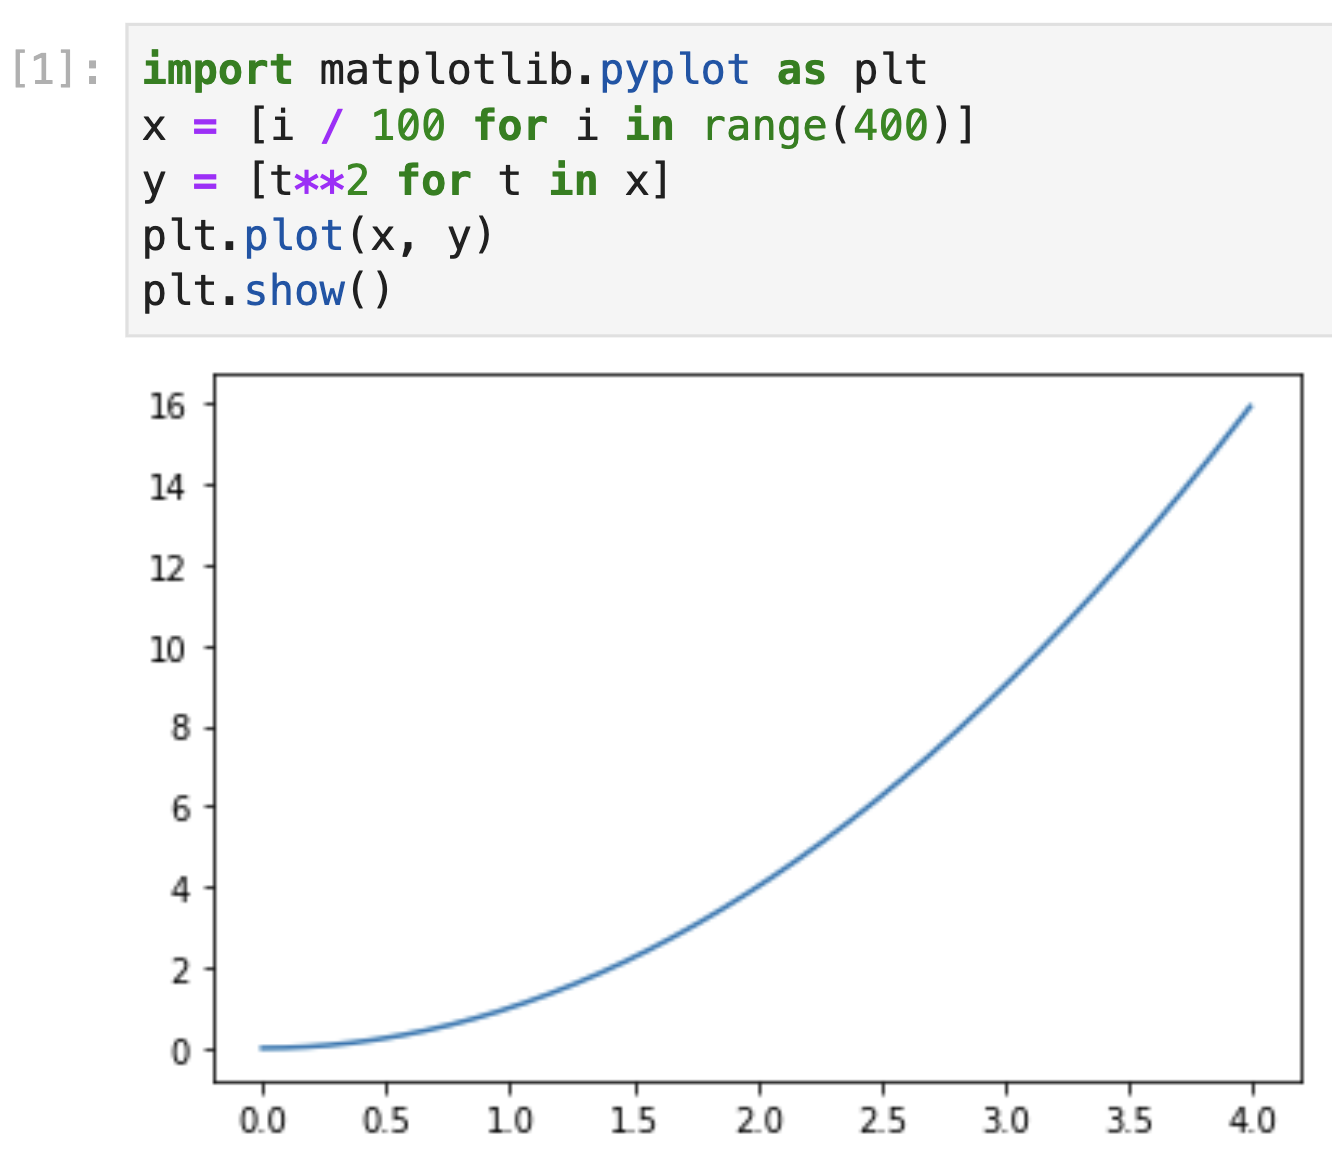
\includegraphics[width=0.9\linewidth]{work/example_matplotlib.png}
\caption{matplotlib でグラフを描画する例} \label{example_matplotlib}
\end{figure}

\subsection{SymPy}
SymPy は、記号計算のための Python ライブラリである。Symbol オブジェクトとして変数を作成し、Eq オブジェクトとして方程式を定義できる。subs 関数を使うことで、作成した方程式に数値を代入することができる。図~\ref{example_sympy} は、SymPy で Equation を定義し、数値を代入する例である。

\begin{figure}[bht]
\centering
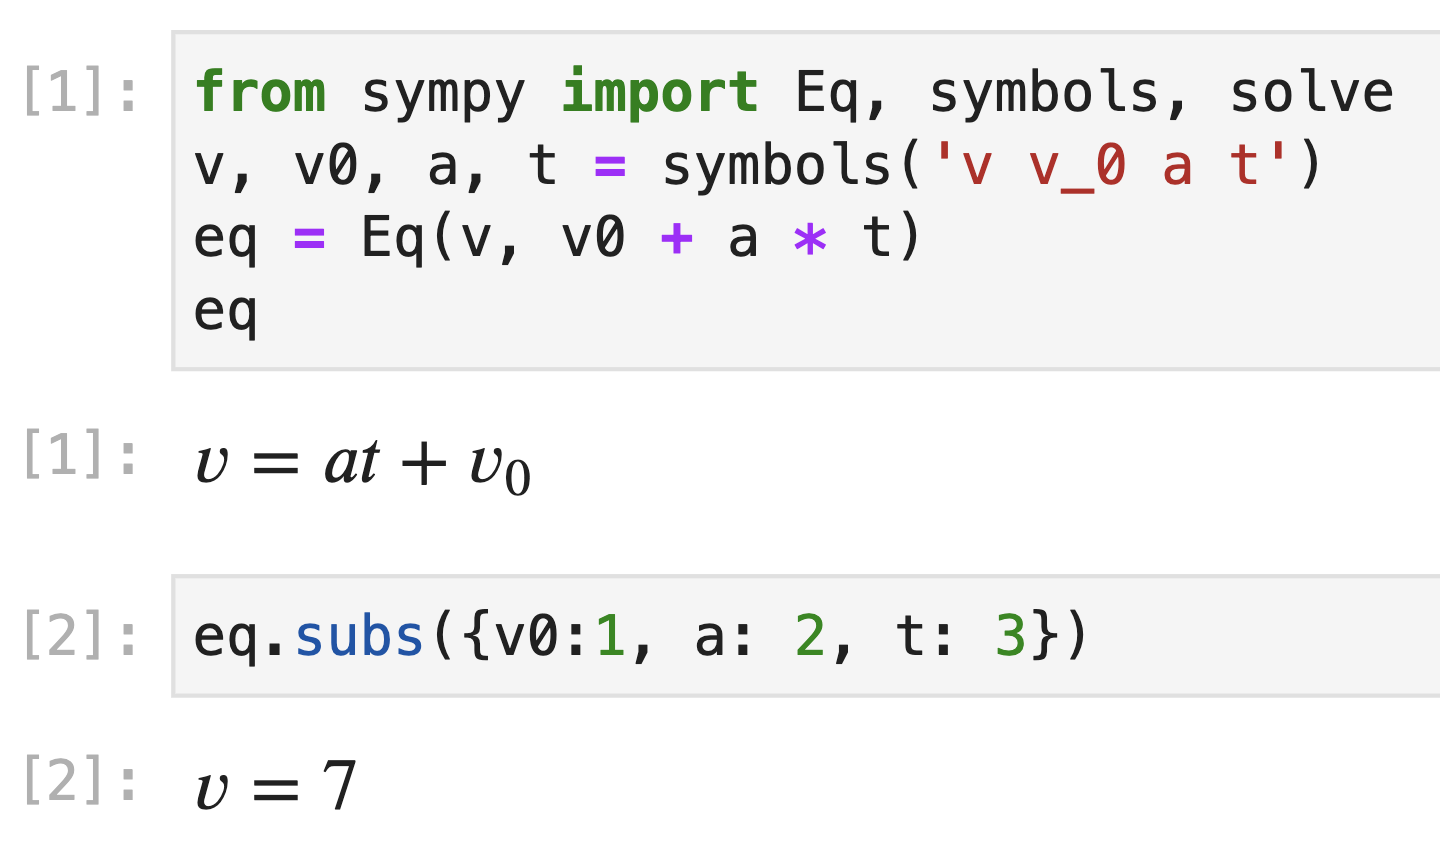
\includegraphics[width=0.9\linewidth]{work/example_sympy.png}
\caption{SymPy で Equation を定義し、数値を代入する例} \label{example_sympy}
\end{figure}

\newpage
\section{処理の流れ}
以下では、学習者の操作によって \simname がどのように物理系を定義しているかを簡単に説明する。

\begin{enumerate}
  \item 学習者が Jupyter 上の Widget に物体名を入力すると、\simname はその物体に紐づく変数を SymPy の Symbol として生成する。生成された変数は Jupyter 上に表示される。
  \item 学習者が物体と動作例を選択すると、\simname は動作例に応じた変数を Symbol として生成し、動作例の運動を表す Sympy の Equation を生成する。
  \item 生成された変数を利用した方程式を学習者が Jupyter 上の Widget に入力すると、\simname はそれを Equation として解釈する。またこの際、不正な次元の方程式になっていないかを確認する。 \label{未実装1}
  \item \simname は、選択された物体の座標・速度などを数値計算するために数値を与える必要のある変数を推論し、それらを入力するための Widget を生成する。 \label{未実装2}
  \item 学習者が数値を入力すると、Equation に数値が代入される。同時に動作例を表す Equation にも数値が代入され、matplotlib を用いて破線で描画される。
  \item 学習者が再生ボタンを押すと、時刻を表す変数 $t$ が時間変化し、物体の位置や座標が再計算され、matplotlib を用いて描画される。
\end{enumerate}

\subsection{実装できていない部分}

先述した \simname の機能のうち、
\begin{itemize}
  \item 学習者の入力を Equation として解釈する (\ref{未実装1}.)
  \item 不正な次元の方程式になっていないかを確認する (\ref{未実装1}.)
  \item 数値計算するために数値を与える必要のある変数を推論する (\ref{未実装2}.)
\end{itemize}
という部分が未実装である。それぞれについて方針を述べる。

\subsubsection*{学習者の入力を Equation として解釈する}
入力の解釈は、sympy.parsing.sympy\_parser の parse\_expr 関数を使うことで可能である。この関数では、文字列を SymPy のSymbol, Sum, Mul や Eq などに変換できる。実際に行う例を図~\ref{example_parse}に示す。一方、単にこれを用いるだけでは未定義の変数を使うことができてしまう。そのため、解釈された変数が定義されたものなのかを確認する必要がある。また、学習者がアンダースコアなどを入力する必要があったり、意図しない解釈をされる($v_Ax$ と $v_{Ax}$ など)可能性がある。Jupyter に表示されている変数をクリックすることでその変数を入力することができれば、このような誤りは防止でき、学習者の入力にかかる手間も減らすことができる。

\begin{figure}[htb]
  \centering
  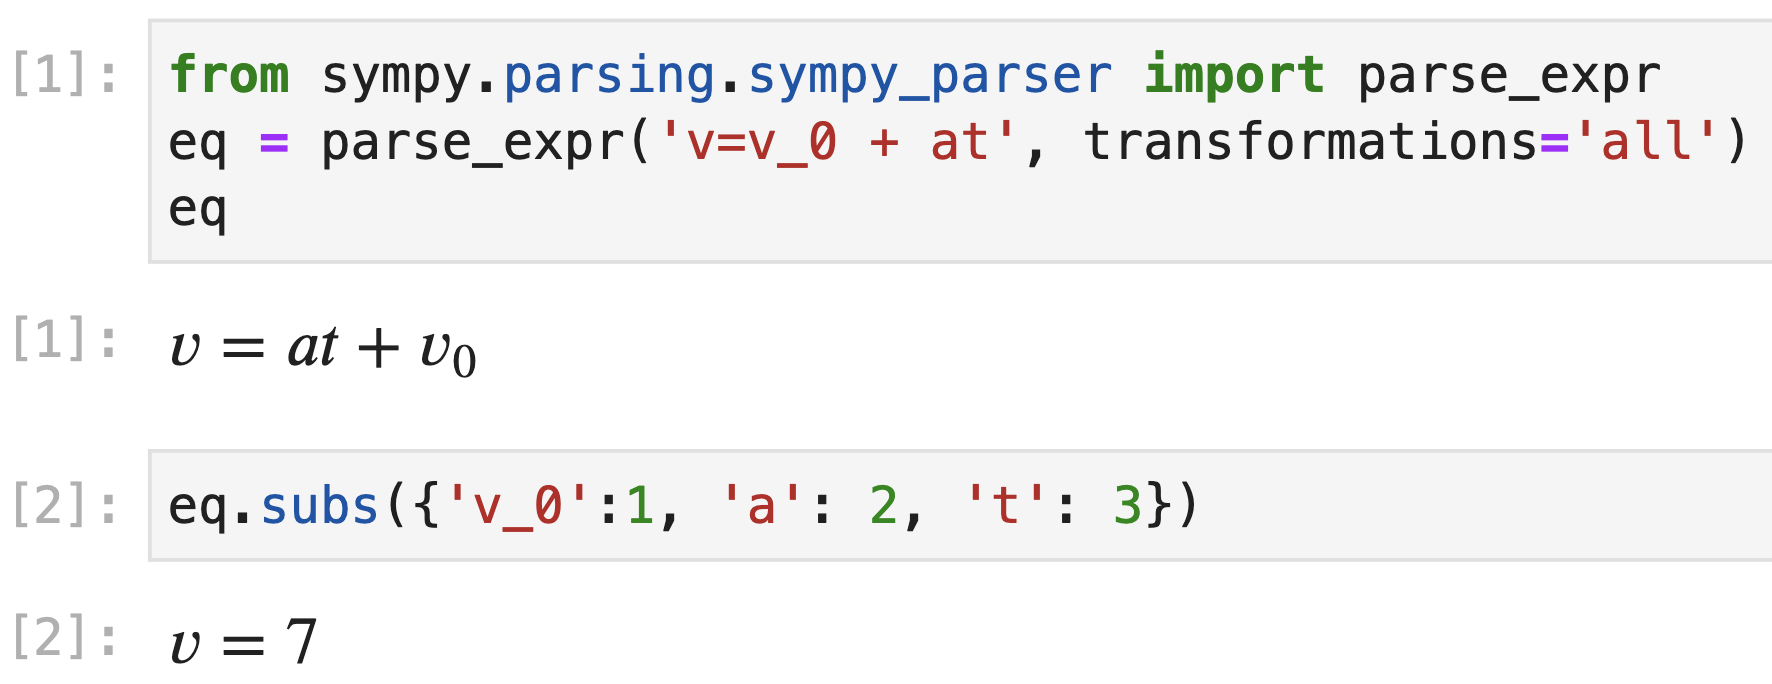
\includegraphics[width=0.9\linewidth]{work/example_parse.png}
  \caption{parse\_expr 関数で文字列をパースする例} \label{example_parse}
\end{figure}

\subsubsection*{不正な次元の方程式になっていないかを確認する}
現在の実装では、 $g + t~~\mathrm{([L/T^2] + [T])}$ のように次元が不正な方程式も定義できてしまう。SymPy の変数に次元の情報を付加し、異なる次元間の加減などを検出する必要がある。自動で追加される変数は生成する際に次元の情報を付加すればよいが、学習者が新たに追加する変数については次元を手動で指定する必要がある。L, M, T などの組み合わせを文字列で入力したものを解釈する、各次元の指数を数値で入力したものを解釈するなどの方法が考えられる。

\subsubsection*{数値計算するために数値を与える必要のある変数を推論する}
基本的には、学習者が定義した方程式に含まれる変数のうち物体に紐づいている位置・速度以外の変数の値を入力させれば良い。しかし、次のような場合も存在する。
\begin{align*}
x_A = X
X = v_0t
\end{align*}
ここで、$x_A$ は物体の $x$ 座標を表す変数で、$X$ と $v_0$ は学習者が定義した変数である。先述した方針では、$X$ と $v_0$ に値を入力する必要がある。しかし実際は $X$ か $v_0$ の一方にのみ値を入力すればよい。このような場合に対応する方法を考える必要がある。